% Imposta lo spazio in orizzontale all'inizio di ogni paragrafo
\setlength{\parindent}{20pt}
\documentclass[12pt, letterpaper]{article}
\usepackage{lipsum} % Pacchetto per generare testo fittizio
\usepackage{graphicx}
\usepackage[letterpaper,top=2cm,bottom=2cm,left=3cm,right=3cm,marginparwidth=1.75cm]{geometry}
\usepackage{amsmath}
\usepackage{xcolor}
\usepackage[colorlinks=true, allcolors=blue]{hyperref}
\usepackage{floatrow} % Pacchetto per gestire la posizione delle didascalie
\usepackage{wrapfig}


\begin{document}
\title{\textbf{Relazione sui circuiti}}
\author{Stefano Doria \and Giuseppe Luciano}
\date{Aprile 2024}

\maketitle

\section{Abstract}
In questa relazione vengono presentati i risultati dell'esperimento condotto sui circuiti elettrici.

\section{Introduzione}

In questo esperimento abbiamo analizzato la variazione di ampiezza e la fase della differenza di potenziale ai capi di un resistore in funzione delle frequenze, utilizzando un circuito con doppio filtro notch. Il filtro notch, nel nostro caso costituito da un condensatore e induttore in parallelo, è progettato per attenuare selettivamente una specifica frequenza lasciando inalterate le altre. Questo avviene poichè alle frequenze prossime a quelle proprie del sistema l'impedenza del blocco risulta essere minima facendo dissipare la quasi totalità dell’energia sul filtro che quindi attenua le ampiezze, come descritto da [METTI ARTICOLO NOTCH]. La larghezza del notch, ossia la larghezza della banda di frequenza attorno alla frequenza di risonanza dove l'attenuazione è significativa, dipende dai valori numerici delle componenti L e C e dal fattore di qualità, come risulta evidente nella funzione di trasferimento del circuito  $H(\omega) = \frac{R(\omega^2 LC-1)}{R(\omega^2 LC -1) -i(\omega L)}$
Il circuito completo, visibile in Figura 1, è costituito da due filtri separati in serie da una resistenza ai capi della quale sono state prese le misure della differenza di potenziale che veniva generato in modo sinusoidale ad una frequenza variabile dalla scheda Elvis II. Così attraverso un programma di acquisizione Labview siamo riusciti ad ottenere i grafici della differenza di fase e dell’ampiezza dell’onda per resistenze diverse. 
\begin{figure}[h]
\floatbox[{\capbeside\thisfloatsetup{capbesideposition={right,bottom}}}]{figure}[\FBwidth]
{\caption{la foto mostra lo schema del circuito costituito da un doppio filtro notch separato in serie da una resistenza}\label{fig:figura}}
{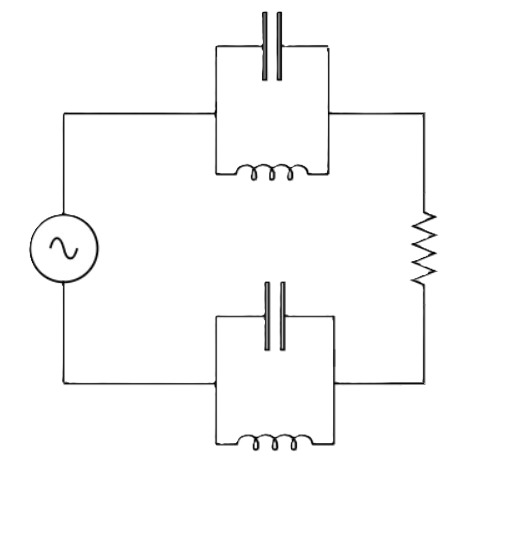
\includegraphics[width=0.6\linewidth]{circuito.jpeg}}
\end{figure}

\section{Metodo Sperimentale}
\subsection{Apparato sperimentale}
Per l'esperimento, volto ad analizzare il comportamento dell'ampiezza e della fase della differenza di potenziale in un circuito costituito da un doppio filtro notch,  sono state condotte diverse valutazioni sulle specifiche dei componenti da impiegare. In particolare, sono stati selezionati due capacitori e due induttori in modo che le frequenze di risonanza dei filtri fossero sufficientemente distanziate evitando in questo modo influenze reciproche e facilitando l’analisi dei dati. 
Nonostante ci fosse stata fornita un’indicazione sui valori nominali delle specifiche tecniche dei vari componenti abbiamo deciso di indagare meglio l’effettivo comportamento degli stessi mediante misure ripetute. Per farlo ci siamo avvalsi del multimetro digitale incorporato nella scheda Elvis II. Questo strumento ci ha permesso di tarare il fondoscala dell'acquisizione in base al valore da misurare, garantendo così risultati più precisi.
METTI COSE DATI
Sono state poi selezionate diverse resistenze, al fine di analizzare il comportamento del sistema per cambiamenti nelle suddette METTI COSE DATI.
Infine per determinare l'ampiezza e la differenza di fase tra il segnale generato dalla scheda Elvis e quello misurato ai capi della resistenza nel nostro circuito, abbiamo utilizzato un programma LabVIEW in grado di campionare alla frequenza desiderata con un numero di punti per acquisizione variabile. In particolare, abbiamo impostato la frequenza di campionamento a circa 20'000 Hz e il numero di punti a (100?).
Il programma LabVIEW era inoltre in grado di comunicare con il function generator della scheda Elvis II, consentendoci di variare la frequenza del segnale generato dopo aver acquisito un numero di campioni sufficiente. Questo ci ha permesso di stimare agevolmente gli errori associati a ciascuna misura e di ottenere valutazioni migliori sugli errori.

\begin{wrapfigure}{r}{0.4\textwidth}
    \centering
    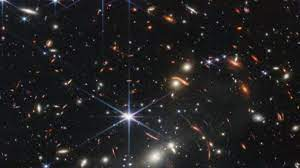
\includegraphics[width=0.38\textwidth]{apparato_sperimentale.jpeg}
    \caption{Qui ci va la descrizione della figura}
    \label{fig:figura}
\end{wrapfigure}

 
\subsection{Svolgimento}
Si è iniziato conducendo diverse analisi per determinare i componenti più adatti per il nostro circuito per poi verificare, dopo una rapida misurazione delle grandezze coinvolte, con l’oscilloscopio da banco che il risultato effettivo fosse in sintonia con le nostre previsioni e che il fenomeno fosse facilmente osservabile. Una volta aver selezionato la componente si è passati ad una valutazione più attenta delle proprietà dell’elemento con il multimetro digitale della scheda Elvis II effettuando diverse misurazioni al fine di incrementare la precisione. 

Successivamente, abbiamo allestito il circuito sulla breadboard incorporata sulla scheda Elvis II, come visibile in Figura 1 assicurandoci che i collegamenti fossero saldi e impostando in configurazione differenziale i due canali di acquisizione per minimizzare effetti causati da possibile rumore. Ciò ci ha inoltre permesso di ridurre l'errore sistematico dovuto alla non simultaneità di acquisizione dei canali a causa della presenza di un solo convertitore analogico-digitale (ADC) che, richiedendo tempo per effettuare la conversione, ritardava quella del secondo canale.

 // a me non fa impazzire scriverlo per intero ma ho letto come sia buona norma mettere il significato di ogni sigla quando citata la prima volta

Successivamente, dopo aver valutato quali valori ci permettessero di ottenere risultati accurati in accordo con il teorema di Nyquist, abbiamo impostato dal computer il sampling rate e il numero di punti da acquisire insieme al passo dell’incremento della frequenza dell'onda generata dalla scheda Elvis. Si è dunque avviata l'acquisizione, durante la quale si è monitorato dinamicamente le figure di Lissajous e le ampiezze per controllare la corretta evoluzione sistema.
Per valutare analiticamente il comportamento del sistema, abbiamo proceduto analizzando le impedenze di ogni singolo filtro per poi sommare il totale. Nello specifico, indicando con $j$ l'unità immaginaria al fine di evitare possibili confusioni, abbiamo ottenuto che $Z_c = \frac{1}{j \omega C}$ e $Z_l = j \omega L$. Considerando poi che tali componenti erano poste in parallelo, abbiamo ottenuto come impedenza complessiva $Z_f= \frac{j\omega L}{1 - \omega^2 LC}$. Quindi, considerando anche la resistenza per un singolo filtro, abbiamo ottenuto un'impedenza totale di
$A= \frac{\sqrt{(\omega L)^2 + [R(\omega^2 LC -1)]^2}}{|\omega^2 LC -1|} \exp\left(\frac{R(\omega^2 LC -1)}{\omega L}\right) $
dove $\phi = \arctan\left(\frac{\omega L}{R(\omega^2 LC -1)}\right)$.

Ottenendo quindi dalla legge di Ohm simbolica un'espressione dell'ampiezza data da
\[
A(\omega)= R \frac{|\omega^2 LC -1|}{\sqrt{(\omega L)^2 + [R(\omega^2 LC -1)]^2}}
\]

\section{Risultati}

ecco come si fanno le tabelle

\begin{table}[htbp]
  \begin{tabular}{|c|c|c|}
    \hline
    Colonna 1 & Colonna 2 & Colonna 3 \\
    \hline
    Elemento 1 & Elemento 2 & Elemento 3 \\
    \hline
    Elemento 4 & Elemento 5 & Elemento 6 \\
    \hline
  \end{tabular}
   \textcolor{gray}{\caption{Esempio di tabella colorato }}
  \label{tab:esempio}
\end{table}

\subsection{Acquisizione dati}
Riportare l’esito delle misure dirette (utilizzando eventualmente anche
delle tabelle).

\subsection{Elaborazione dati}
Riportare le analisi statistiche di misure ripetute, le misure indirette, i
risultati dei fit, le correzioni per effetti sistematici. Mettere in evidenza i
risultati principali dell’esperimento.

\section{Conclusioni}
Riassumere i risultati ottenuti ed eventualmente confrontarli con le previsioni
della teoria e/o con misure sperimentali precedenti (se esistono).
Discutere i possibili effetti sistematici non corretti che potrebbero essere causa
di differenze tra valore misurato e valore atteso (evitando però ipotesi non
giustificate).

\section{Biografia}
Riferimenti bibliografici e fonti consultate.

\section{Appendice}
Eventuali dettagli aggiuntivi o dati supplementari.

\end{document}

